\section*{Задание 1. Одноканальная система в форме вход-выход}

Имеем данное дифференциальное уравнение:
\begin{equation*}
    \dddot y + 9\ddot y + 26\dot y + 24 y = 2\ddot u +6\dot u +8 u,
\end{equation*}
преобразуем его немного:
\begin{equation*}
    p^3y=2p^2u+6pu+8u-9p^2y-26py-24y,
\end{equation*}
% \begin{equation*}
%     y=\frac{1}{p}2u+\frac{1}{p^2}6u+\frac{1}{p^3}8u-\frac{1}{p}9y-\frac{1}{p^2}26y-\frac{1}{p^3}24y,
% \end{equation*}
\begin{equation*}
    y=\frac{1}{p^3}[2p^2[u]+6p[u]+8u-9p^2[y]-26p[y]-24y],
\end{equation*}
\begin{equation*}
    y=\frac{1}{p^3}[2\ddot u+6\dot u+8u-9\ddot y-26\dot y-24y].
\end{equation*}
Моделирование (см. схему на рисунке \ref{fig:task_1_slx}) для $u(t)=1$ и 
нулевым начальных условиях можно увидеть на рисунке \ref{fig:task_1_y} - график сигнала $y(t)$,
график сигнала $u(t)$ очевиден - константа, так что его график опущен.

\begin{figure}[htbp]
    \centering
    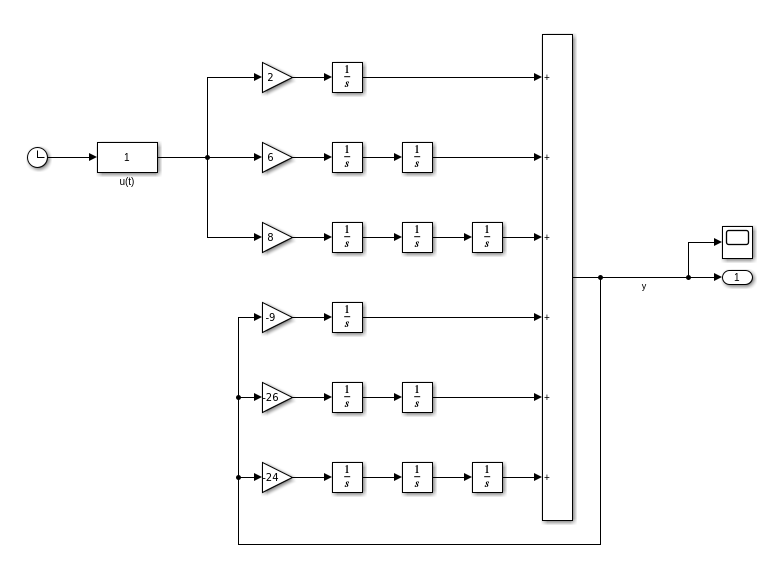
\includegraphics[width=\linewidth]{figs/task_1_slx.png}
    \caption{Структурная схема системы для задания 1.}
    \label{fig:task_1_slx}
\end{figure}

\begin{figure}[htbp]
    \centering
    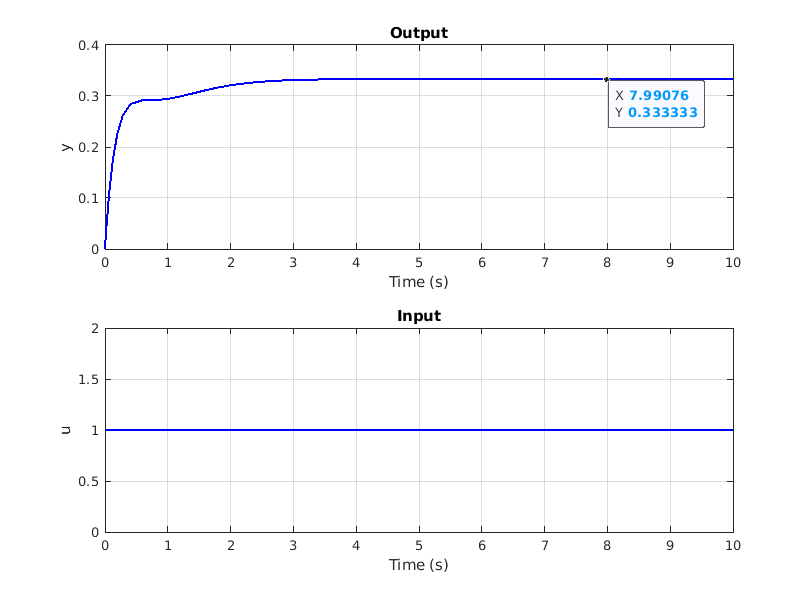
\includegraphics[width=0.7\linewidth]{figs/task_1_out.png}
    \caption{График сигнала $y(t)$ для задания 1.}
    \label{fig:task_1_y}
\end{figure}




\section*{Задание 2. Переход от формы вход-выход к форме вход-состояние-выход}

Для системы из Задания 1 определим передаточную функцию $W(p)$ (ПФ):
$$
(p^3+9p^2+26p+24)[y]=(2p^2+6p+8)[u],
$$
\begin{equation}
    \label{eq:pf1}
    W(p)=\frac{2p^2+6p+8}{p^3+9p^2+26p+24}.
\end{equation}
Построим  математические модели вход-состояние-выход (В-С-В):
\begin{equation*}
    \begin{cases}
        \dot x = Ax + Bu,\\
        y = Cx + Du.
    \end{cases}
\end{equation*}

\begin{enumerate}
    \item Каноническая управляемая форма. Структурную схему можно увидеть
    на рисунке \ref{fig:task2_slx_ctrl}, а график выхода на рисунке 
    \ref{fig:task2_out_ctrl_y}.
\begin{equation*}
    \begin{array}{cc}
        A_y=\begin{bmatrix}
            0 & 1 & 0 \\
            0 & 0 & 1 \\
            -24 & -26 & -9
        \end{bmatrix}, &
        B_y=\begin{bmatrix}
            0 \\ 0 \\ 1
        \end{bmatrix}, \\[7mm]
        C_y=\begin{bmatrix}
            8 & 6 & 2
        \end{bmatrix}, &
        D_y=0.
    \end{array}
\end{equation*}
\begin{figure}[htbp]
    \centering
    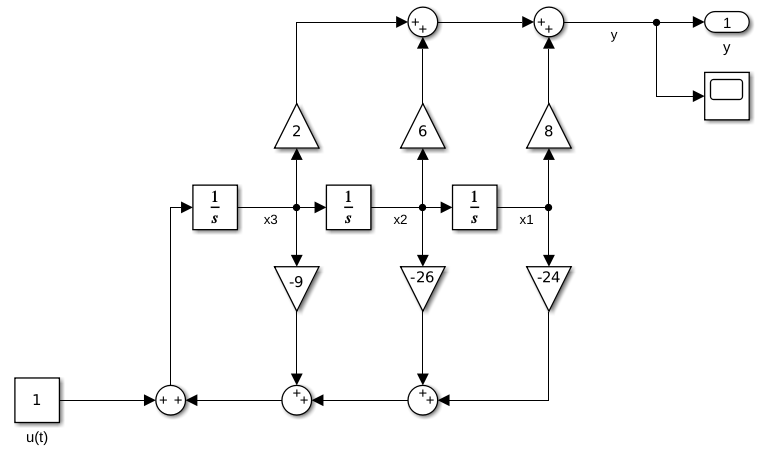
\includegraphics[width=\linewidth]{figs/task_2_slx_ctrl.png}
    \caption{Структурная схема канонической управляемой формы.}
    \label{fig:task2_slx_ctrl}
\end{figure}
\begin{figure}[htbp]
    \centering
    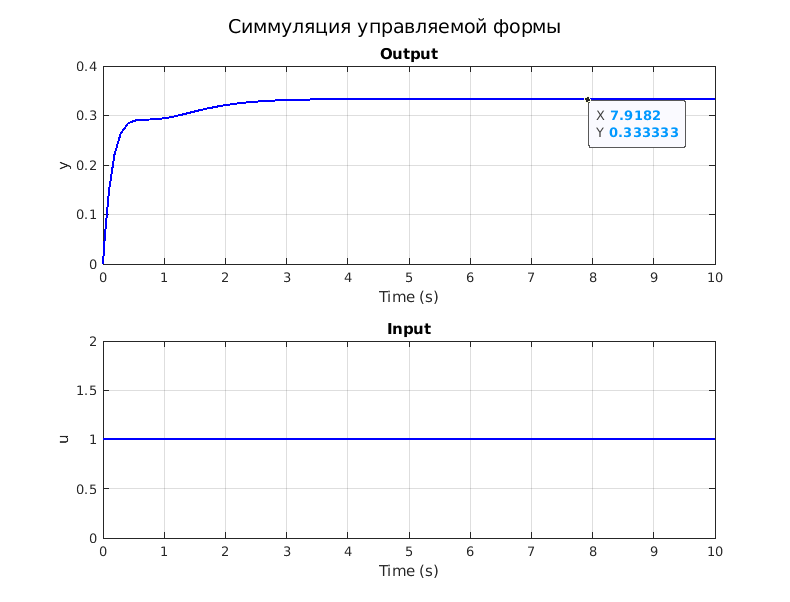
\includegraphics[width=0.7\linewidth]{figs/task_2_out_ctrl_y.png}
    \caption{Графики сигнала $y(t)$ канонической управляемой формы.}
    \label{fig:task2_out_ctrl_y}
\end{figure}

    \item Каноническая наблюдаемая форма.Структурную схему можно увидеть
    на рисунке \ref{fig:task2_slx_wtch}, а график выхода на рисунке 
    \ref{fig:task2_out_wtch_y}.
    \begin{equation*}
        \begin{array}{cc}
            A_\text{н}=\begin{bmatrix}
                0 & 0 & -24 \\
                1 & 0 & -26 \\
                0 & 1 & -9
            \end{bmatrix}, &
            B_\text{н}=\begin{bmatrix}
                8 \\ 6 \\ 2
            \end{bmatrix}, \\[7mm]
            C_\text{н}=\begin{bmatrix}
                0 & 0 & 1
            \end{bmatrix}, &
            D_\text{н}=0.
        \end{array}
    \end{equation*}
    \begin{figure}[htbp]
        \centering
        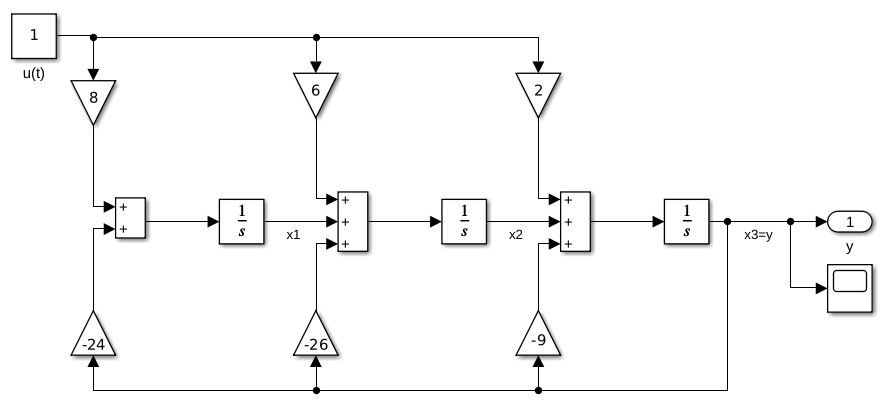
\includegraphics[width=\linewidth]{figs/task_2_slx_wtch.png}
        \caption{Структурная схема канонической наблюдаемой формы.}
        \label{fig:task2_slx_wtch}
    \end{figure}
    \begin{figure}[htbp]
        \centering
        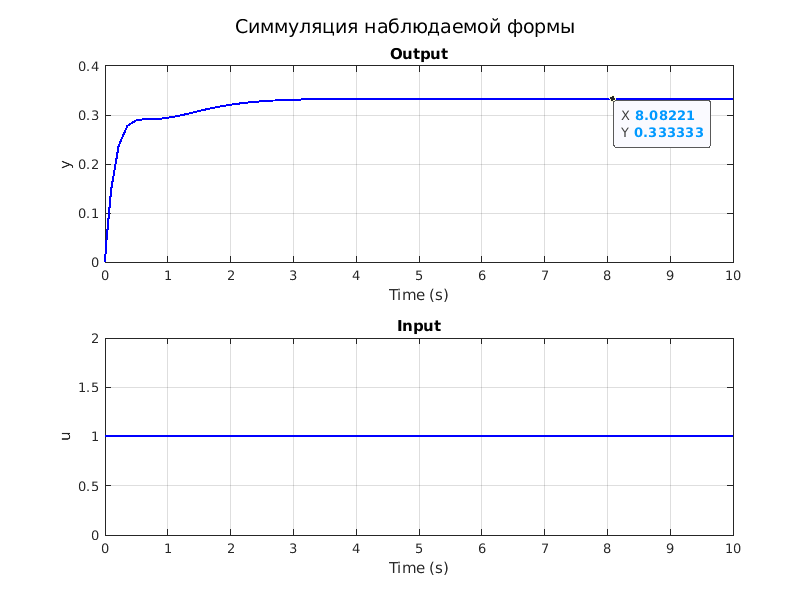
\includegraphics[width=0.7\linewidth]{figs/task_2_out_wtch_y.png}
        \caption{Графики сигнала $y(t)$ канонической наблюдаемой формы.}
        \label{fig:task2_out_wtch_y}
    \end{figure}

    \item Каноническая диагональная форма.Структурную схему можно увидеть
    на рисунке \ref{fig:task2_slx_diag}, а график выхода на рисунке 
    \ref{fig:task2_out_diag_y}.
    Для начала разобъем ПФ из уравнения \ref{eq:pf1} на простые дроби и получим
    \begin{equation*}
        \frac{2}{p+2}-\frac{8}{p+3}+\frac{8}{p+4}.
    \end{equation*}
    Теперь можем получить матрицы:
    \begin{equation*}
        \begin{array}{cc}
            A_\text{Д}=\begin{bmatrix}
                -2 & 0 & 0 \\
                0 & -3 & 0 \\
                0 & 0 & -4
            \end{bmatrix}, &
            B_\text{Д}=\begin{bmatrix}
                2 \\ -8 \\ 8
            \end{bmatrix}, \\[7mm]
            C_\text{Д}=\begin{bmatrix}
                1 & 1 & 1
            \end{bmatrix}, &
            D_\text{Д}=0.
        \end{array}
    \end{equation*}
    \begin{figure}[htbp]
        \centering
        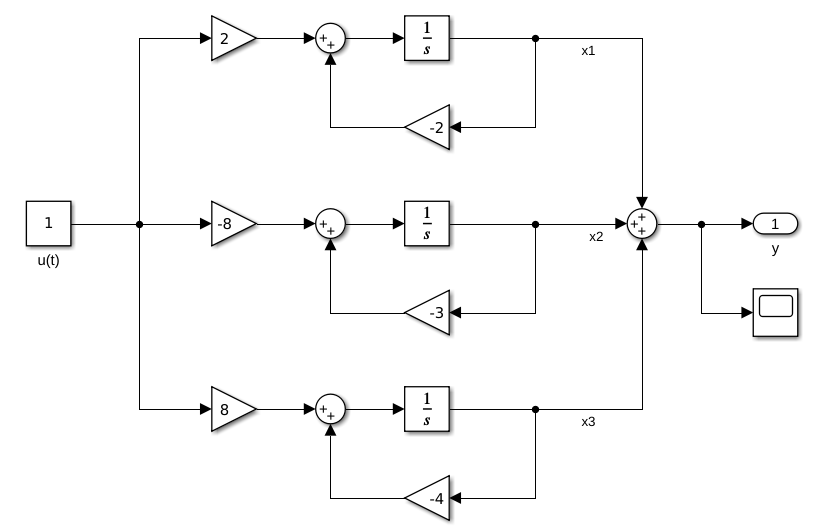
\includegraphics[width=\linewidth]{figs/task_2_slx_diag.png}
        \caption{Структурная схема канонической диагональной формы.}
        \label{fig:task2_slx_diag}
    \end{figure}
    \begin{figure}[htbp]
        \centering
        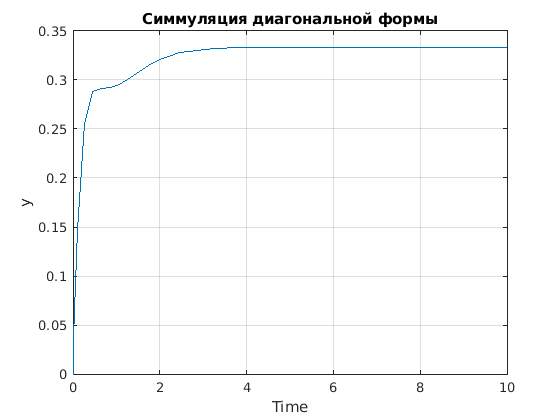
\includegraphics[width=0.7\linewidth]{figs/task_2_out_diag_y.png}
        \caption{Графики сигнала $y(t)$ канонической диагональной формы.}
        \label{fig:task2_out_diag_y}
    \end{figure}
\end{enumerate}

Графики моделирования канонических форм имеют одинаковые графики выхода,
но заметим, что они отличаются от первоначального графика из задания 1,
а отличаются только более резким ростом и "ямкой" перед выходом
у уствновившемуся значению, и не понятно, от чего эти различия.



\section*{Задание 3. Многоканальная система в форме вход-выход}

В соответствии с моим вариантом рассмотрим систему
\begin{equation*}
    A(p)y(y)=B(p)u(t),
\end{equation*}
где
\begin{equation*}
    \begin{array}{cc}
        A(p)=\begin{bmatrix}
            p+17&p+5\\
            p+4&p+2
        \end{bmatrix}, &
        B(p)=\begin{bmatrix}
            6&8\\4&3
        \end{bmatrix}.        
    \end{array}
\end{equation*}
Передаточная матрица (ПМ) для данной системы будет равна
\begin{equation*}
    W(p)=A^{-1}(p)B(p),
\end{equation*}
для ее нахождения найдем обратную матрицу $A(p)$:
\begin{equation*}
    A^{-1}(p)=\frac{1}{10p+14}\begin{bmatrix}
        p+2&-p-5\\-p-4&p+17
    \end{bmatrix},
\end{equation*}
тогда ПМ будет равна
\begin{equation*}
    W(p)=\frac{1}{10p+14}\begin{bmatrix}
        2p-8&5p+1\\-2p+44&-5p+19
    \end{bmatrix}.
\end{equation*}


Для того чтобы подготовить систему для симуляции в SIMULINK, раскроем матричное уравнение.
Пусть $y(t)=\begin{bmatrix}y_1(t)\\y_2(t)\end{bmatrix}$, 
а $u(t)=\begin{bmatrix}u_1(t)\\u_2(t)\end{bmatrix}$.
Теперь распишем систему дифференциальных уравнений:
\begin{equation*}
    \begin{array}{c}
        (p+17)y_1(t)+(p+5)y_2(t)=6u_1(t)+8u_2(t),\\[2mm]
        p[y_1(t)]+17y_1(t)+p[y_2(t)]+5y_2(t)=6u_1(t)+8u_2(t),\\[2mm]
        y_1(t)=\frac{1}{p}6u_1(t)+\frac{1}{p}8u_2(t)-\frac{1}{p}5y_2(t)-\frac{1}{p}17y_1(t)-y_2(t),
    \end{array}
\end{equation*}
так же
\begin{equation*}
    \begin{array}{c}
        (p+4)y_1(t)+(p+2)y_2(t)=4u_1(t)+3u_2(t),\\[2mm]
        p[y_1(t)]+4y_1(t)+p[y_2(t)]+2y_2(t)=4u_1(t)+3u_2(t),\\[2mm]
        y_2(t)=\frac{1}{p}4u_1(t)+\frac{1}{p}3u_2(t)-\frac{1}{p}2y_2(t)-\frac{1}{p}4y_1(t)-y_1(t).
    \end{array}
\end{equation*}
Я попытался сделать структурную схему, которую можно увидеть на рисунке 
\ref{fig:task3_slx}, но SIMULINK не захотел нормально это чудо симулировать,
сначало говорил, что имеется сингулярность, при уменьшении шага все посчитал, но
графики $y_1(t)$ и $y_2(t)$ выдал какие-то невменяемые, на них ничего не видно.
\begin{figure}[htbp]
    \centering
    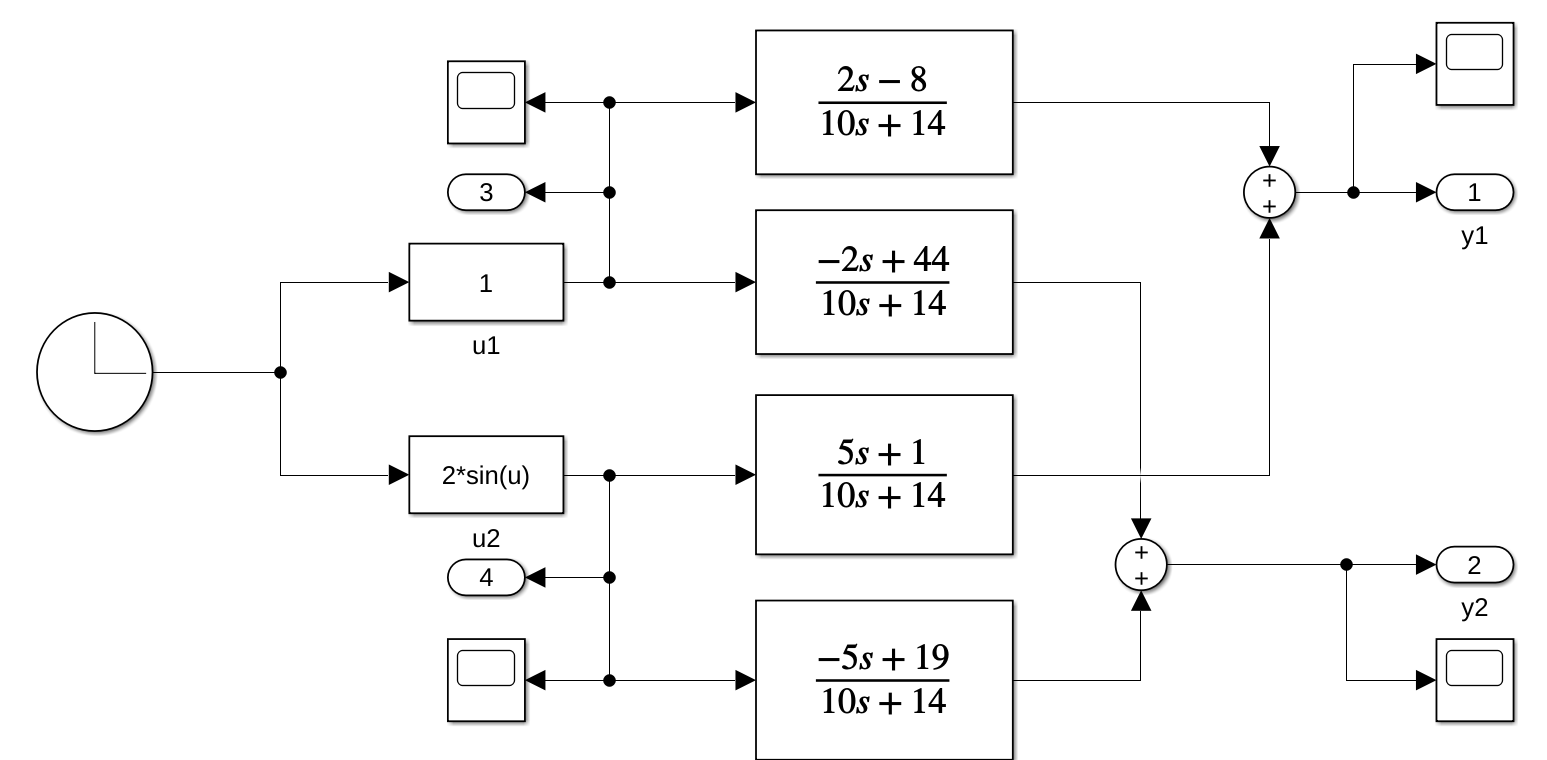
\includegraphics[width=1\linewidth]{figs/task_3_slx.png}
    \caption{Структурная схема задания 3.}
    \label{fig:task3_slx}
\end{figure}



\section*{Задание 4. Многоканальная система в форме вход-состояние-выход}

Имеем матрицы MIMO системы
\begin{equation*}
    \begin{array}{ccc}
        A=\begin{bmatrix}
            0&-2\\1&-7
        \end{bmatrix},&
        B=\begin{bmatrix}
            3&0\\2&7
        \end{bmatrix},&
        C=\begin{bmatrix}
            0&7\\4&6
        \end{bmatrix}.
    \end{array}
\end{equation*}
Для дальнейшего построения структурной схемы раскроем матричное произведение:
\begin{equation*}
    \begin{array}{c}
        \dot x_1=-2x_2+3u_1,\\[2mm]
        x_1=\frac{1}{p}[3u_1-2x_2],
    \end{array}
\end{equation*}
\begin{equation*}
    \begin{array}{c}
        \dot x_2=x_1-7x_2+2u_1+7u_2,\\[2mm]
        x_2=\frac{1}{p}[2u_1+7u_2-7x_2-x_1].
    \end{array}
\end{equation*}
Получившуюся схему можно увидеть на рисунке \ref{fig:task4_slx}, а графики входа,
вывода и состояния системы можно увидеть на рисунке \ref{fig:task4_out}.
\begin{figure}[htbp]
    \centering
    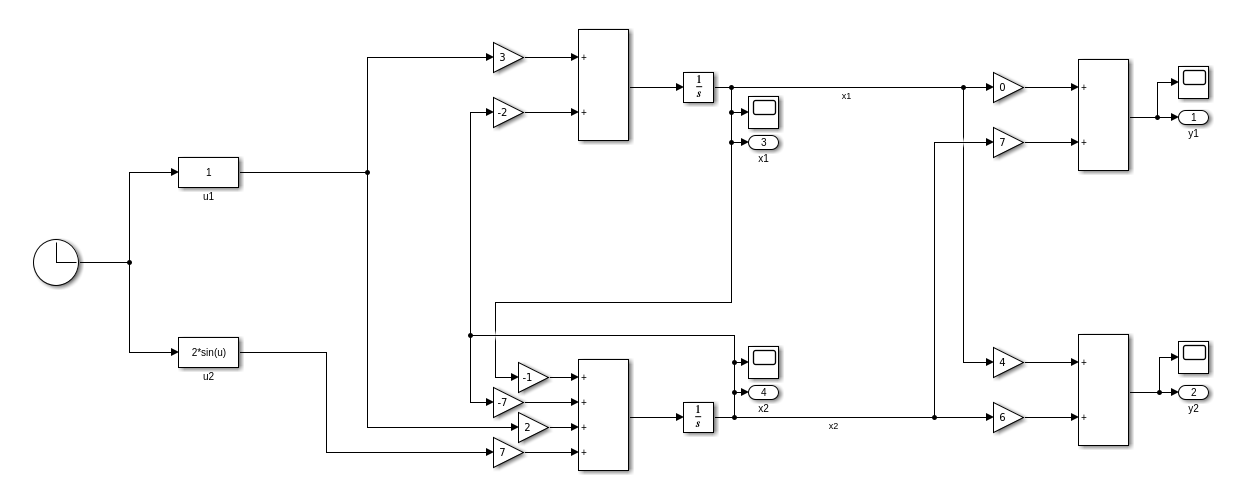
\includegraphics[width=1\linewidth]{figs/task_4_slx.png}
    \caption{Структурная схема задания 4.}
    \label{fig:task4_slx}
\end{figure}

\begin{figure}[htbp]
    \centering
    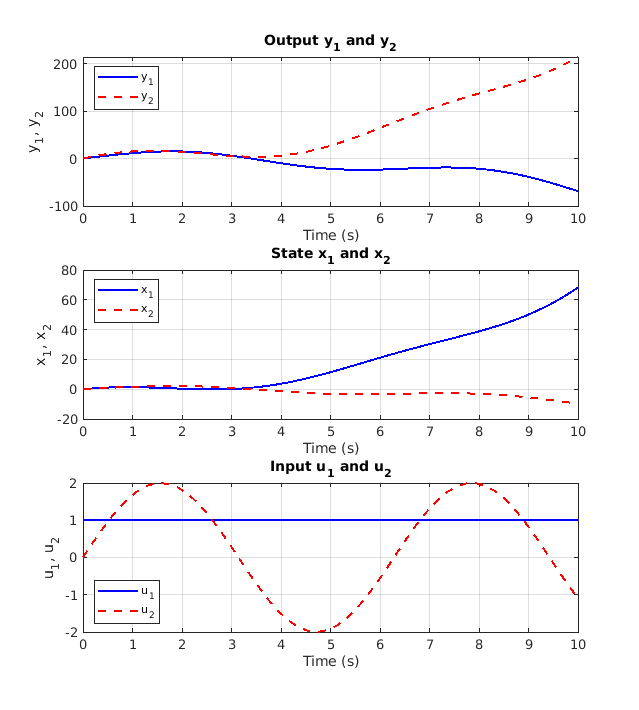
\includegraphics[width=1\linewidth]{figs/task_4_out.png}
    \caption{Графики входа, вывода и состояния системы из задания 4.}
    \label{fig:task4_out}
\end{figure}